\startSolutions{trans2}{Linear Transformations on $\R^2$}

\begin{enumerate}[!HW!, start=1]
\begin{multicols}{4}
\itemspade %$\mtx{rr}{1&0\\0&5}\mtx{cr}{1/2&0\\0&1} = 
$\mtx{cc}{1/2&0\\0&5}$
\itemspade %$\mtx{rr}{1&0\\2&1}\mtx{cc}{1&0\\0&5} = 
$\mtx{cc}{1&0\\2&5}$
\itemspade %$\mtx{rr}{-1&0\\0&-1}\mtx{cc}{0&1\\1&0} = 
$\mtx{rr}{0&-1\\-1&0}$
\itemspade %$ \mtx{rr}{0&1\\1&0}\mtx{rr}{5&0\\0&1}\mtx{rr}{-1&0\\0&1} = 
$\mtx{rr}{0&1\\-5&0}$
\end{multicols}
\itemspade %$\mtx{rr}{1&0\\0&3}\mtx{rr}{1&0\\-2&1}\mtx{cc}{\sqrt{3}/2&-1/2\\1/2&\sqrt{3}/2} = 
$\dfrac{1}{2}\mtx{cc}{\sqrt{3}&-1\\3-6\sqrt{3}&6+3\sqrt{3}}$

\itemspade $\mtx{rr}{4&0\\0&1}$\\ Stretch horizontally by a factor of $4$. %Devan Hill
\begin{center}
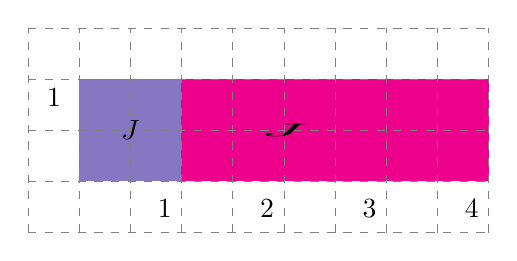
\begin{tikzpicture}[scale=0.65]
%\fill[cyan] (0,0) rectangle (2,2);
\fill[magenta] (0,0) -- (8,0) -- (8,2) -- (0,2) -- cycle;
\fill[magenta!50!cyan] (0,0) rectangle (2,2);
\draw[help lines,dashed] (-1,-1) grid (8,3);
\node at (1,1) {$J$};
\begin{scope}[cm={4,0,0,1,(0,0)}]
\node[transform shape] at (1,1) {$J$};
\end{scope}
\gridlines{-1}{9}{-1}{3};
\node[below left, yshift=-3] at (2,0) {$1$};
\node[below left, yshift=-3] at (4,0) {$2$};
\node[below left, yshift=-3] at (6,0) {$3$};
\node[below left, yshift=-3] at (8,0) {$4$};
\node[below left, xshift=-3] at (0,2) {$1$};
\end{tikzpicture}
\end{center}

\itemspade $\mtx{rr}{1&0\\0&-1}\mtx{rr}{1&0\\0&8}$\\
Stretch vertically by a factor of $8$ and reflect across the $x$-axis.
\begin{center}
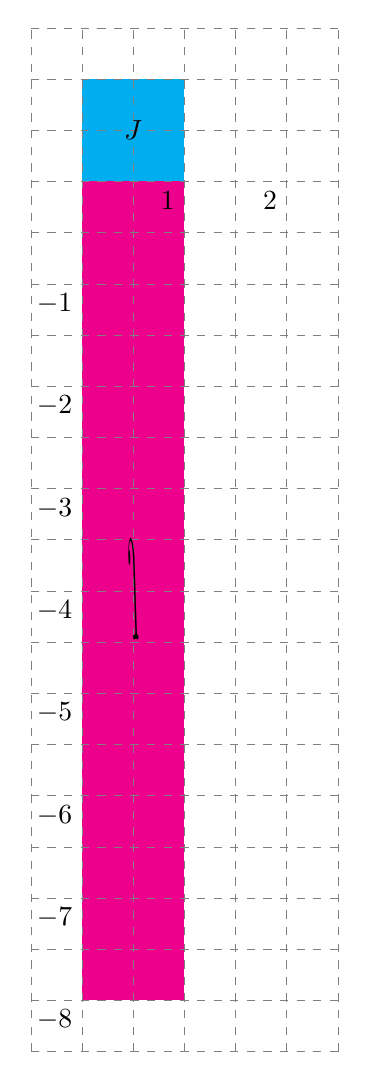
\begin{tikzpicture}[scale=0.65]
\fill[cyan] (0,0) rectangle (2,2);
\fill[magenta] (0,0) rectangle (2,-16);
\begin{scope}
\clip (0,0) rectangle (2,2);
\end{scope}
\draw[help lines,dashed] (-1,-17) grid (5,3);
\node at (1,1) {$J$};
\begin{scope}[cm={1,0,0,-8,(0,0)}]
\node[transform shape] at (1,1) {$J$};
\end{scope}
\gridlines{-1}{5}{-17}{3};
\node[below left] at (2,0) {$1$};
\node[below left] at (0,-2) {$-1$};
\node[below left] at (0,-4) {$-2$};
\node[below left] at (0,-6) {$-3$};
\node[below left] at (0,-8) {$-4$};
\node[below left] at (0,-10) {$-5$};
\node[below left] at (0,-12) {$-6$};
\node[below left] at (0,-14) {$-7$};
\node[below left] at (0,-16) {$-8$};
\node[below left] at (4,0) {$2$};
\end{tikzpicture}
\end{center}

\itemspade  $\mtx{rr}{0&1\\1&0}\mtx{rr}{4&0\\0&1}\mtx{rr}{1&0\\0&2}\mtx{rr}{1&0\\0&-1}$\\
Reflect across the $x$-axis, stretch vertically by a factor of $2$, stretch horizontally by a factor of $4$, and reflect across the line $y=x$.
\begin{center}
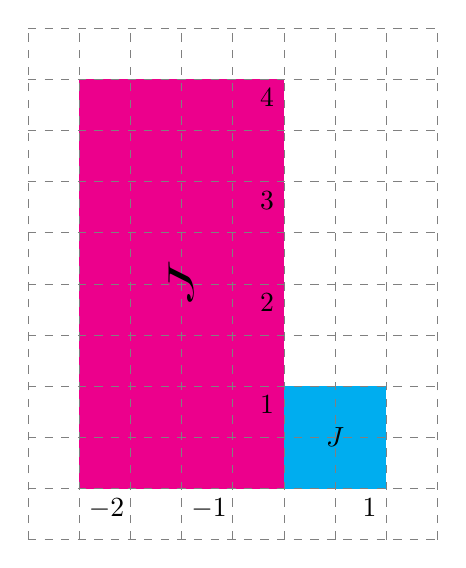
\begin{tikzpicture}[scale=0.65]
\fill[cyan] (0,0) rectangle (2,2);
\fill[magenta] (0,0) -- (0,8) -- (-4,8) -- (-4,0) -- cycle;
\draw[help lines,dashed] (-5,-1) grid (3,9);
\node at (1,1) {$J$};
\begin{scope}[cm={0,4,-2,0,(0,0)}]
\node[transform shape] at (1,1) {$J$};
\end{scope}
\gridlines{-5}{3}{-1}{9};
\node[below left] at (2,0) {$1$};
\node[below right] at (-2,0) {$-1$};
\node[below right] at (-4,0) {$-2$};
\node[below left] at (0,2) {$1$};
\node[below left] at (0,4) {$2$};
\node[below left] at (0,6) {$3$};
\node[below left] at (0,8) {$4$};
\end{tikzpicture}
\end{center}

\itemspade $\mtx{rr}{3&0\\0&1}\mtx{rr}{1&6\\0&1}\mtx{rr}{1&0\\0&13}\mtx{rr}{1&-2\\0&1}$\\
Shear horizontally by a factor of $-2$, stretch vertically by a factor of $13$, shear vertically by a factor of $6$, and stretch horizontally by a factor of $3$.
\begin{center}
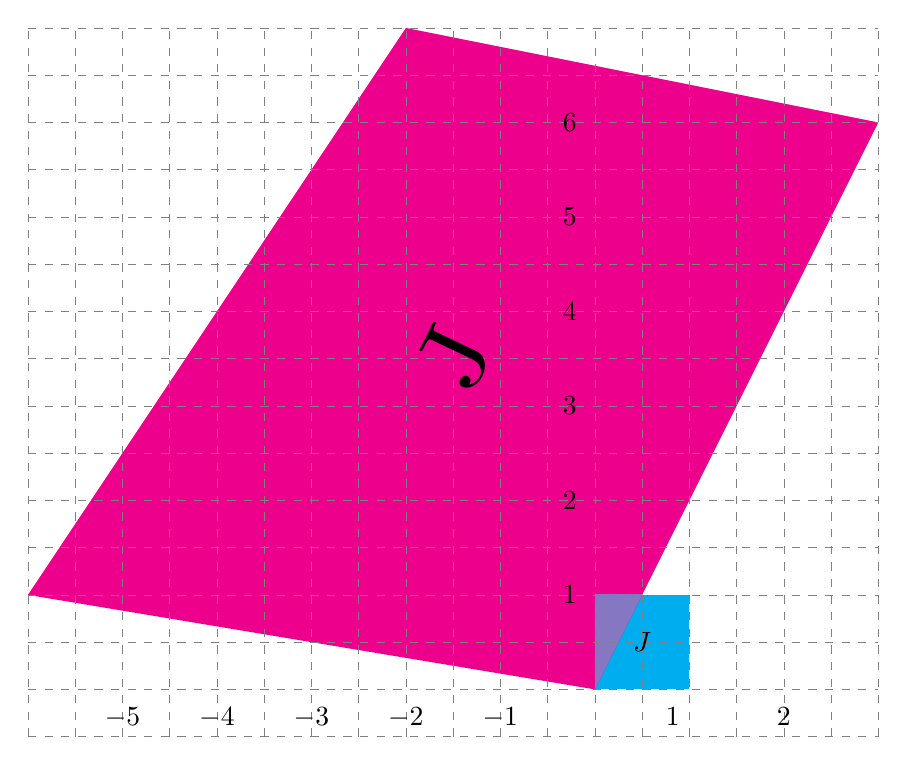
\begin{tikzpicture}[scale=0.6]
\fill[cyan] (0,0) rectangle (2,2);
\fill[magenta] (0,0) -- (6,12) -- (-4,14) -- (-12,2) -- cycle;
\begin{scope}
\clip (0,0) rectangle (2,2);
\fill[magenta!50!cyan] (0,0) -- (6,12) -- (-4,14) -- (-12,2) -- cycle;
\end{scope}
\draw[help lines,dashed] (-12,-1) grid (6,14);
\node at (1,1) {$J$};
\begin{scope}[cm={3,6,-6,1,(0,0)}] %List Columns first
\node[transform shape] at (1,1) {$J$};
\end{scope}
\gridlines{-12}{6}{-1}{14};
\node[below left, yshift=-3] at (2,0) {$1$};
\node[below, yshift=-3] at (-2,0) {$-1$};
\node[below, yshift=-3] at (-4,0) {$-2$};
\node[below, yshift=-3] at (-6,0) {$-3$};
\node[below, yshift=-3] at (-8,0) {$-4$};
\node[below, yshift=-3] at (-10,0) {$-5$};
\node[below, yshift=-3] at (4,0) {$2$};
\node[left, xshift=-3] at (0,2) {$1$};
\node[left, xshift=-3] at (0,4) {$2$};
\node[left, xshift=-3] at (0,6) {$3$};
\node[left, xshift=-3] at (0,8) {$4$};
\node[left, xshift=-3] at (0,10) {$5$};
\node[left, xshift=-3] at (0,12) {$6$};
\end{tikzpicture}
\end{center}

\item $\mtx{rr}{0&-1\\-1&0} = \mtx{rr}{-1&0\\0&-1}\mtx{rr}{0&1\\1&0}$

\itemspade
\begin{enumerate}
\item 
\begin{multline*} \mtx{rr}{\cos \theta & -\sin \theta \\ \sin \theta & \cos \theta}\mtx{rr}{1 & 0 \\ 0 & -1}\mtx{rr}{\cos \theta & -\sin \theta \\ \sin \theta & \cos \theta}^{-1} = \mtx{rr}{\cos \theta & -\sin \theta \\ \sin \theta & \cos \theta}\mtx{rr}{1 & 0 \\ 0 & -1}\mtx{rr}{\cos \theta & \sin \theta \\ -\sin \theta & \cos \theta}\\
= \mtx{rr}{\cos \theta & -\sin \theta \\ \sin \theta & \cos \theta}\mtx{rr}{\cos \theta & \sin \theta \\ \sin \theta & -\cos \theta}
= \mtx{cc}{\cos^2\theta - \sin^2\theta & 2\sin\theta\cos\theta\\ 2\sin\theta\cos\theta & \sin^2\theta - \cos^2\theta}
= \mtx{cc}{\cos2\theta & \sin2\theta \\ \sin2\theta & -\cos2\theta} = A
\end{multline*} 
\item The sequence of geometric transformations in the factorization of $A$ rotates the plane clockwise about the origin by an angle of $\theta$, then reflects the plane across the $x$-axis, then rotates the plane counter-clockwise about the origin by an angle of $\theta$.\\

Since the line $\ell$ is the unique line through the origin that forms an angle of $\theta$ with the $x$-axis, the composite of these transformations moves $\ell$ onto the $x$-axis, reflects across the $x$-axis, and then moves the $x$-axis back to $\ell$. The net effort on the plane is to reflect across the line $\ell$.\\ 
\item $ \mtx{rr}{\cos 2(0) & \sin 2(0) \\ \sin 2(0) & -\cos 2(0)} =  \mtx{rr}{\cos 0 & \sin 0 \\ \sin 0 & -\cos 0} = \mtx{rr}{1 & 0 \\ 0 & -1}$, which is reflection across the $x$-axis, the unique line which forms a $0$ angle with the $x$-axis.\\
$ \mtx{rr}{\cos 2(\pi/4) & \sin 2(\pi/4) \\ \sin 2(\pi/4) & -\cos 2(\pi/4)} =  \mtx{rr}{\cos (\pi/2) & \sin (\pi/2) \\ \sin (\pi/2) & -\cos (\pi/2)} = \mtx{rr}{0 & 1 \\ 1 & 0}$, which is reflection across the line $y=x$, the unique line which forms a $\dfrac{\pi}{4}$ angle with the $x$-axis.\\\\
$ \mtx{rr}{\cos 2(\pi/2) & \sin 2(\pi/2) \\ \sin 2(\pi/2) & -\cos 2(\pi/2)} =  \mtx{rr}{\cos \pi & \sin \pi \\ \sin \pi & -\cos \pi} = \mtx{rr}{-1 & 0 \\ 0 & 1}$, which is reflection across the $y$-axis, the unique line which forms a $\dfrac{\pi}{2}$ angle with the $x$-axis.\\
\item $ \mtx{rr}{\cos 2(\pi/6) & \sin 2(\pi/6) \\ \sin 2(\pi/6) & -\cos 2(\pi/6)} =  \mtx{rr}{\cos (\pi/3) & \sin (\pi/3) \\ \sin (\pi/3) & -\cos (\pi/3)} = \mtx{cc}{1/2 & \sqrt{3}/2 \\ \sqrt{3}/2 & -1/2} = \dfrac{1}{2}\mtx{rr}{1 & \sqrt{3} \\ \sqrt{3} & -1}$
\begin{center}
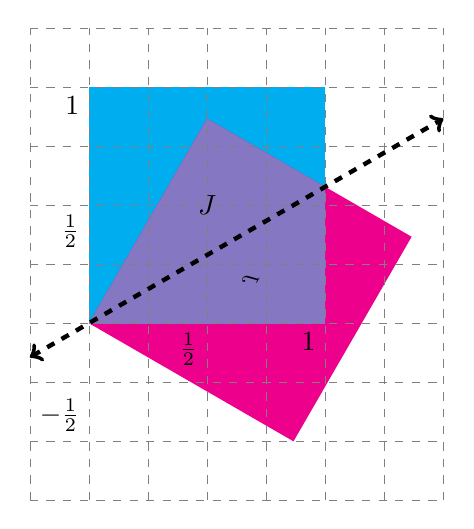
\begin{tikzpicture}[scale=0.75]
\fill[cyan] (0,0) rectangle (4,4);
\fill[magenta] (0,0) -- (2,3.464) -- (5.464,1.464) -- (3.464,-2) -- cycle;
\begin{scope}
\clip (0,0) rectangle (4,4);
\fill[magenta!50!cyan] (0,0) -- (2,3.464) -- (5.464,1.464) -- (3.464,-2) -- cycle;
\end{scope}
\draw[help lines,dashed] (-1,-3) grid (6,5);
\node at (2,2) {$J$};
\begin{scope}[cm={0.5,0.866,0.866,-0.5,(0,0)}]
\node[transform shape] at (2,2) {$J$};
\end{scope}
\gridlines{-1}{6}{-3}{5};
\draw[ultra thick, dashed, <->] (-1,-0.577) -- (6, 3.464);
\node[below left] at (2,0) {$\frac{1}{2}$};
\node[below left] at (4,0) {$1$};
%\node[below left] at (6,0) {$3$};
\node[below left] at (0,2) {$\frac{1}{2}$};
\node[below left] at (0,4) {$1$};
\node[above left] at (0,-2) {$-\frac{1}{2}$};
\end{tikzpicture}
\end{center}
\item 
\begin{multline*}
B = \mtx{rr}{\cos \theta & -\sin \theta \\ \sin \theta & \cos \theta}\mtx{rr}{1 & m \\ 0 & 1}\mtx{rr}{\cos \theta & -\sin \theta \\ \sin \theta & \cos \theta}^{-1} = \mtx{rr}{\cos \theta & -\sin \theta \\ \sin \theta & \cos \theta}\mtx{rr}{1 & m \\ 0 & 1}\mtx{rr}{\cos \theta & \sin \theta \\ -\sin \theta & \cos \theta} \\
= \mtx{rr}{\cos \theta & -\sin \theta \\ \sin \theta & \cos \theta}\mtx{cc}{\cos \theta - m\sin\theta & \sin \theta+m\cos\theta \\ -\sin \theta & \cos \theta} \\
= \mtx{cc}{\cos^2 \theta - m\sin\theta\cos\theta + \sin^2\theta & \sin \theta\cos\theta+m\cos^2\theta -\sin\theta\cos\theta\\ \sin\theta\cos\theta-m\sin^2\theta-\sin \theta\cos\theta & \sin^2\theta+m\sin\theta\cos\theta + \cos^2 \theta} 
= \mtx{cc}{1-\frac{m}{2}\sin2\theta & m\cos^2\theta \\ -m\sin^2\theta & 1 + \frac{m}{2}\sin2\theta}\\ = \dfrac{1}{2}\mtx{cc}{2-m\sin2\theta & m + m\cos2\theta \\ -m+m\cos2\theta & 2 + m\sin2\theta}
\end{multline*} 
\end{enumerate}
\item \begin{proof}
Since $A$ is nonsingular, it can be factored into a product of elementary matrices. Replacement elementary matrices cause shears, scaling elementary matrices cause stretches, compressions, and reflections. Interchange elementary matrices cause reflections.
\end{proof}
\end{enumerate}

\vspace{-15 pt}